
In this chapter the approach to the  characteristics of the satellite system are described. In the upcoming sections all aspects are threaded separately. 

\section{Reliability}
\label{blRAMSrel}
Compared to conventional laser altimetry missions, a swarm of receivers is used in this system. Spreading the receivers over a number of satellites reduces the risk of the mission failing. If one receiver satellite fails there will still be others to perform the task of detecting photons. Using a low-power laser emitter extends the lifetime of the mission compared to missions using a higher power laser, since low-power lasers generally wear out slower. Figure \ref{R} on page \pageref{R} gives a overview of subsystem contributions to satellite failures after different time span from a non-parametric analysis. More detail reliability analysis can be found in chapter risk assessment.
\begin{figure} [H]
	\begin{center}
         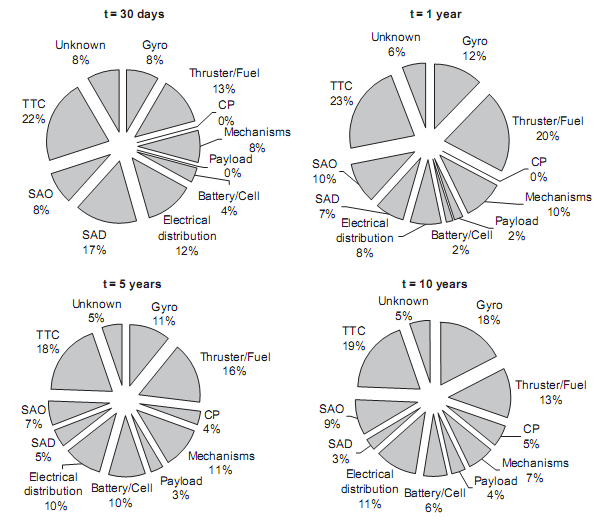
\includegraphics[width=1.0\textwidth,angle=0]{chapters/img/subsystem_reliability_analysis.png}
	
	\caption{Subsystem contributions to satellite failures after 30 days, 1 year, 5 years, and 10 years in-orbit.\cite{reliability}}
	\label{R}
	\end{center}
	\end{figure}

\section{Availability}
\label{blRAMSavail}
The system is designed functional all the time to cover the entire Earth. To safe power it is also possible of switch off the laser to only make measurements in a designated area. Since the system use a swarm of receivers the system can still make measurements if some of the receivers in pointed in the wrong direction.

\section{Maintainability}
\label{blRAMSmaint}
Maintainability is defined as the ability of our operating system specific item to be maintained. In our case, as with most other satellite missions, it is not possible to do regular on-board maintenance to the satellites themselves. The main focus in maintenance is on the ground segment and can be divided in two parts: preventive maintenance and corrective maintenance. They are considering separately as follows: 
	\begin{enumerate}
		\item Preventive maintenance. During the regular system operation time, there are periodic maintenance and condition dependent maintenance.  System software or simulator servicing maintenance of ground station is mandatory and data link rate needs to be adjusted in some cases. On the other hand, conditional maintenance is set to do some specific inspections to prevent something going wrong in the future.
		\item Corrective maintenance. This is mainly carried out after something goes wrong. For instance, if one of the photon receiver is not functional, the system can relocate the rest of the receivers to decrease the functional influence mostly. But if the laser emitter is broken, it is no way to obtain the maintenance. Corrective maintenance is also used during analyzing measurements data to obtain better resolution or accuracy.
  	\end{enumerate}
Since the mission consists of a swarm of satellites it will be possible to add more satellites to the swarm, for example to upgrade the mission or extend the mission life. 

\section{Safety}
\label{blRAMSsaf} 
The system safety is mainly considered during launch and decommissioning. The safety risks during launch are mainly covered by choosing a reliable launcher. For decommission it is important to choose a decent orbit in such a way that it ensures the satellite to burn up in the atmosphere entirely. Most of the time the satellite is on its orbit in space. The orbits of the satellites need to be designed in such a way that they will not intervene with the orbits of other satellites, even when the satellite fails. 